\section{Experiment}
\textbf{Experimental Setup.} We evaluated several popular open-source vision-language models (VLMs), including Qwen2VL~\cite{wang2024qwen2}, Qwen2.5VL~\cite{bai2025qwen2}, InternVL2.5~\cite{bai2025qwen2}, LLaVA-Video~\cite{zhang2024videoinstructiontuningsynthetic}, NVILA~\cite{liu2024nvila}, and VideoLLaMA3~\cite{zhang2025videollama}, alongside the closed-source Gemini-2.5 and GPT-4o accessed via API. All models were prompted identically to generate detailed video descriptions across 21 dimensions. For better evaluation, we adopted two  powerful LLM (\eg, Gemini-2.5-Pro-Preview and GPT-4.1) as TextQA experts to answer VCapsBench questions based on the generated descriptions. The evaluation metrics, derived from their responses, are presented in Table.~\ref{tab:results_1} and Appendix~\ref{exp_app} Table.~\ref{tab:results_2}. Following the Playground v3 protocol~\cite{playgroundv3}, each caption was queried three times, and a consensus response was obtained to minimize output variability and ensure consistency.


\begin{figure}[thbp]
	\begin{minipage}[t]{1.0\linewidth}
        \centering
	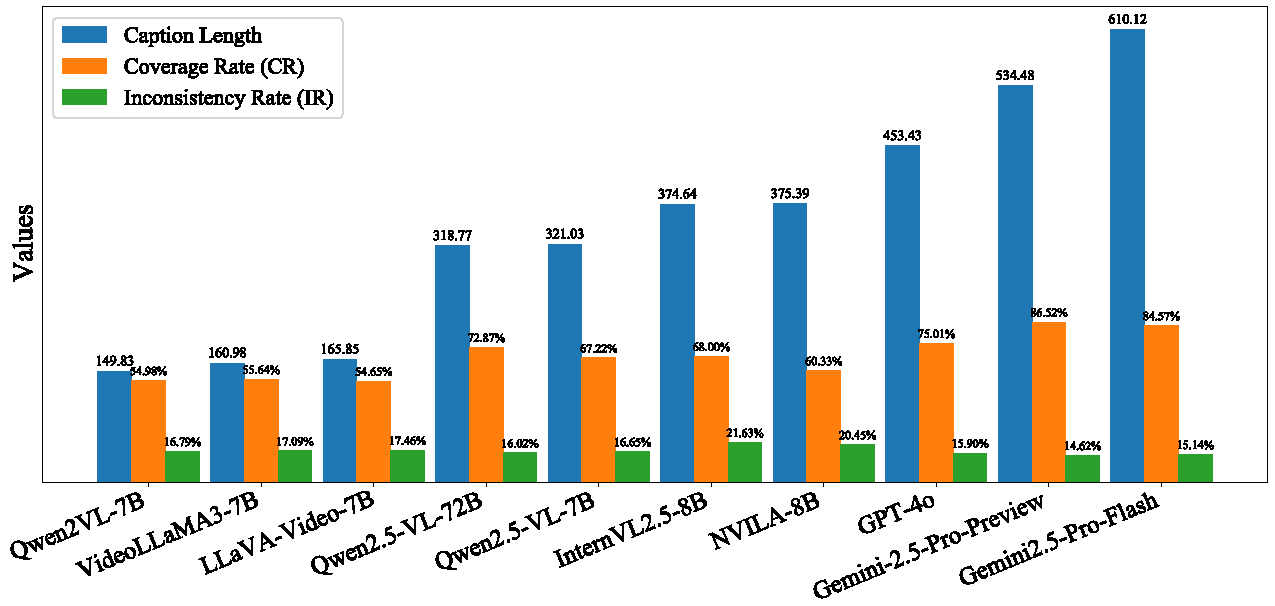
\includegraphics[width=1.0\linewidth]{imgs/comparison_chart_sorted_NEW11.pdf}
    \vspace{-0.5em}
	\caption{The relationship between CR, IR and caption length, where Gemini-2.5-Pro-Preview as a TextQA expert. Caption length is the number of words in the caption, not counting special symbols.}
	\label{fig:fig7}
	\end{minipage}%
	\vspace{-1.5em}	
\end{figure}


\subsection{Main Results}

\textbf{Accuracy (AR):} As illustrated in Table~\ref{tab:results_1} and Fig.~\ref{fig:fig6}, Gemini-2.5-Pro-Preview consistently surpasses all other models across various dimensions when evaluated using the Accuracy (AR) metric. For instance, in the ``Content \& Entity" dimension, specifically concerning action, Gemini-2.5-Pro-Preview achieves an AR of 74.13\%, whereas other models typically fall between 40\% and 70\%. In the ``Color \& Light" dimension, particularly for lighting, Gemini-2.5-Pro-Preview records an impressive AR of 79.67\%, significantly outperforming its counterparts. When considering the entire dataset, Gemini-2.5-Pro-Preview achieves an AR of 73.88\%, which is markedly superior to that of other open-source models. Among these, the latest Qwen2.5-VL-72B shows the best performance with an AR of 61.20\%, yet it remains considerably lower than Gemini-2.5-Pro-Preview. This underscores Gemini-2.5-Pro-Preview's exceptional ability to accurately capture and describe video content, thereby delivering higher quality descriptions and insights.


\textbf{Inconsistency Rate (IR):} Gemini-2.5-Pro-Preview stands out in terms of the IR metric, achieving the lowest IR values. For instance, in the ``Visuals \& Composition'' category, especially for background, Gemini-2.5-Pro-Preview records an IR of just 9.76\%, while other models typically range between 10\% and 20\%. In the ``Cinematography \& Environment'' category, especially for lighting, Gemini-2.5-Pro-Flash's IR is only 14.22\%.

\textbf{Coverage Rate (CR):} When it comes to the CR metric, Gemini-2.5-Pro-Preview again shows superior performance. In the ``Content \& Entity'' category, the lowest CR for Gemini-2.5-Pro-Preview is 61.12\% in the ``Entity Shape'' subcategory, while the highest is 90.12\% in the ``Entity'' subcategory. Other open-source models have CR values that are more than 10\% lower across all categories. Overall, Gemini-2.5-Pro-Preview achieves an impressive CR of 86.52\%. Among open-source models, InternVL2.5-8B performs best with a CR of 68.00\%, which is 18.52\% lower than Gemini-2.5-Pro-Preview. This demonstrates that Gemini-2.5-Pro-Preview can cover more relevant content from the video, providing more comprehensive coverage regardless of description consistency. 

Gemini-2.5-Pro-Preview excels in generating video descriptions, demonstrating high accuracy (AR), consistency (IR), and comprehensive coverage (CR). This underscores its superior performance in producing high-quality, detailed, and consistent descriptions compared to other models. VCapsBench highlights the shortcomings of existing open-source VLMs, such as the lack of detailed object shapes, sizes, colors, and lighting in descriptions. These deficiencies can be particularly problematic for applications requiring highly detailed and complete captions, such as text-to-video generation models and advanced video analysis tools.


\subsection{Evaluation Analysis}
Although Gemini surpasses open-source VLMs in every aspect, showcasing its advanced video comprehension abilities, it is crucial to acknowledge that Gemini's captions were utilized in creating QA-pairs, potentially influencing its elevated CR. Nevertheless, Gemini's metrics are valuable as they establish a benchmark for open-source models, emphasizing the disparity in video content understanding. This insight is instrumental in guiding the optimization of open-source VLMs.

\begin{figure*}[thbp]
	\begin{minipage}[t]{1.0\linewidth}%\centering
	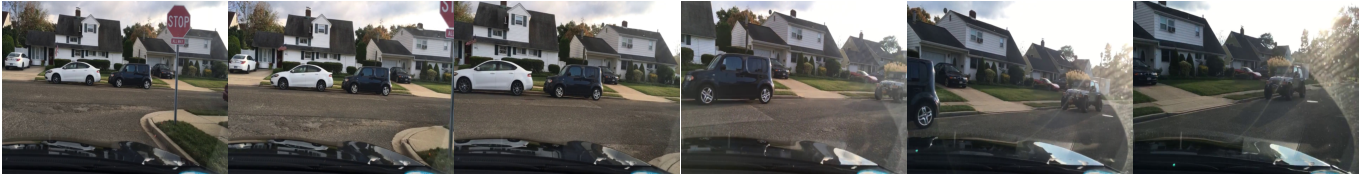
\includegraphics[width=1\linewidth]{imgs/exp_video3.pdf}
    \vspace{-1.5em}
     \caption{Representative video from VCapsBench.}
	\label{fig:fig9}
	\end{minipage}%
	\vspace{-1.5em}	
\end{figure*}

\begin{table*}[htbp]
\centering
\setlength{\tabcolsep}{6pt}
\renewcommand{\arraystretch}{0.8}
\caption{Questions for representative video from VCapsBench. ``Q2.5-72B", ``LV-7B", ``Q2-7B", ``VL-7B", ``NV-8B", ``I2.5-8B", ``Q2.5-7B", ``G2.5" represent ``Qwen2.5VL-72B", ``LLaVA-Video-7B", ``Qwen2VL-7B", ``VideoLLaMA3-7B", ``NVILA-8B", ``InternVL2.5-8B", ``Qwen2.5VL-7B" and ``Gemini-2.5-Pro-Preview" respectively. ``\CheckmarkBold", ``\XSolidBrush", ``\boldmath $\bullet$" represent ``Positive", ``Negative" and ``Unanswerable", respectively.}
\resizebox{\textwidth}{!}{%
\begin{tabular}{l|l|p{9.2cm}|c|cccccccc}
\toprule 
    % &Category & Question & GT & \begin{tabular}[c]{@{}c@{}}\small Qwen2VL\\ \small 72B\end{tabular} & 
    % \begin{tabular}[c]{@{}c@{}}\small LLaVA\\ \small Video-7B\end{tabular} & \begin{tabular}[c]{@{}c@{}}\small Qwen2VL\\ \small 7B\end{tabular} & \begin{tabular}[c]{@{}c@{}}\small VideoLLaMA3\\ \small 7B\end{tabular}
    % & \begin{tabular}[c]{@{}c@{}}\small NVILA\\ \small 8B\end{tabular} & \begin{tabular}[c]{@{}c@{}}\small InternVL2.5\\ \small 8B\end{tabular}& \begin{tabular}[c]{@{}c@{}}\small Qwen2.5VL\\ \small 7B\end{tabular} & \small Gemini-1.5\\ 
    &Category & Question & GT & \small Q2.5-72B &\small LV-7B& \small Q2-7B & \small VL-7B
    & \small NV-8B & \small I2.5-8B & \small Q2.5-7B & \small G2.5\\ 
    \midrule
    \multirow{7}{*}{\rotatebox{90}{\begin{tabular}[c]{@{}c@{}}\small Content\\ \small  \& Entity \end{tabular} }}
    &action & Is there a subtle panning movement from left to right in the video? & yes & \CheckmarkBold & \XSolidBrush & \XSolidBrush & \CheckmarkBold & \boldmath $\bullet$ & \CheckmarkBold & \CheckmarkBold & \CheckmarkBold\\
    \cline{2-4} 
    &count & Are there more than three cars visible in the video? & yes & \boldmath $\bullet$ &  \CheckmarkBold &  \CheckmarkBold & \CheckmarkBold & \CheckmarkBold & \CheckmarkBold & \CheckmarkBold & \CheckmarkBold\\
    \cline{2-4} 
    &relation & Is the red car parked on the opposite side of the street? & yes & \boldmath $\bullet$ &  \boldmath $\bullet$& \CheckmarkBold  & \boldmath $\bullet$ & \boldmath $\bullet$ &\XSolidBrush &\boldmath $\bullet$ &\XSolidBrush\\
    \cline{2-4} 
    &entity& Is there a stop sign in the video? & yes &  \CheckmarkBold & \CheckmarkBold & \CheckmarkBold & \CheckmarkBold &\CheckmarkBold &\CheckmarkBold &\CheckmarkBold &\CheckmarkBold\\
    \cline{2-4} 
    &entity size & Is the black SUV larger than the white sedan? & yes & \boldmath $\bullet$ &  \boldmath $\bullet$ & \boldmath $\bullet$ &\boldmath $\bullet$  &\boldmath $\bullet$ &\boldmath $\bullet$ &\boldmath $\bullet$ &\boldmath $\bullet$\\
    \cline{2-4} 
    &entity shape& Is the stop sign octagonal? & yes & \boldmath $\bullet$ & \boldmath $\bullet$ & \CheckmarkBold & \boldmath $\bullet$ &\boldmath $\bullet$ & \boldmath $\bullet$ &\boldmath $\bullet$ & \CheckmarkBold\\
     \midrule
    \multirow{6}{*}{\rotatebox{90}{\begin{tabular}[c]{@{}c@{}}\small Color\\ \small  \& Light \end{tabular}}}
    &lighting & \begin{tabular}[l]{@{}l@{}}Is the lighting in video primarily natural and even, \\ characteristic of daytime? \end{tabular}& yes &  \CheckmarkBold & \boldmath $\bullet$ & \XSolidBrush & \boldmath $\bullet$ & \CheckmarkBold & \CheckmarkBold & \CheckmarkBold &  \CheckmarkBold \\
    \cline{2-4} 
    &color palette & Does the video have a realistic color palette? & yes & \CheckmarkBold &  \CheckmarkBold &\boldmath $\bullet$ & \boldmath $\bullet$ & \boldmath $\bullet$ &\CheckmarkBold &\CheckmarkBold &  \CheckmarkBold\\
    \cline{2-4} 
    &color grading & Is the image ungraded, with natural tones for the houses and cars? & yes & \boldmath $\bullet$ &  \CheckmarkBold &\boldmath $\bullet$ & \boldmath $\bullet$ & \boldmath $\bullet$ &\CheckmarkBold & \boldmath $\bullet$  &  \CheckmarkBold \\
    \cline{2-4} 
    &color &Is the white sedan parked directly in front of the stop sign? & yes & \boldmath $\bullet$ &  \boldmath $\bullet$ &  \CheckmarkBold &  \boldmath $\bullet$ & \XSolidBrush & \XSolidBrush & \boldmath $\bullet$ & \boldmath $\bullet$\\
    \midrule
    \multirow{6}{*}{\rotatebox{90}{\begin{tabular}[c]{@{}c@{}}\small Visuals \& \\ \small Composition \end{tabular}}}&position & Is the stop sign on the right side of the road? & yes & \boldmath $\bullet$ & \CheckmarkBold & \CheckmarkBold & \boldmath $\bullet$ & \CheckmarkBold & \CheckmarkBold &\boldmath $\bullet$ & \boldmath $\bullet$\\
    \cline{2-4} 
    &relative position & Is the white car closer to the stop sign than the black car? & no & \boldmath $\bullet$ &  \boldmath $\bullet$ & \XSolidBrush & \boldmath $\bullet$ &\boldmath $\bullet$ &\boldmath $\bullet$ & \boldmath $\bullet$ &\boldmath $\bullet$\\
    \cline{2-4} 
    &background & Is the video set in a residential suburban street? & yes & \CheckmarkBold & \CheckmarkBold & \CheckmarkBold & \CheckmarkBold & \CheckmarkBold & \CheckmarkBold & \CheckmarkBold &  \CheckmarkBold \\
    \cline{2-4} 
    &text & Is there a stop sign with the text ``ALL WAY" in the video? & yes & \CheckmarkBold & \XSolidBrush & \CheckmarkBold   & \CheckmarkBold & \CheckmarkBold & \XSolidBrush & \CheckmarkBold & \boldmath $\bullet$\\
    \cline{2-4} 
    &blur & Is there a shallow depth of field in the video? & yes & \boldmath $\bullet$ &  \CheckmarkBold &\boldmath $\bullet$ & \boldmath $\bullet$ & \boldmath $\bullet$ & \boldmath $\bullet$ & \boldmath $\bullet$ &  \CheckmarkBold \\
    \midrule
    \multirow{3}{*}{\rotatebox{90}{ \begin{tabular}[c]{@{}c@{}}\small Cinematography\\ \small  \& Environment \end{tabular}}}&camera movement & Is the camera movement in the video a slow panning from left to right? & yes & \CheckmarkBold & \XSolidBrush & \XSolidBrush & \CheckmarkBold & \boldmath $\bullet$ & \boldmath $\bullet$ & \XSolidBrush &  \CheckmarkBold\\
    \cline{2-4} 
    &shot type& Is the primary shot type predominantly a medium shot taken from a fixed perspective? & yes & \boldmath $\bullet$ & \XSolidBrush & \XSolidBrush & \boldmath $\bullet$ & \boldmath $\bullet$ & \XSolidBrush & \XSolidBrush &  \CheckmarkBold \\
    \cline{2-4} 
    &atmosphere & Is the video set in a calm and quiet atmosphere, typical of a residential neighborhood?  & yes & \CheckmarkBold & \CheckmarkBold  & \CheckmarkBold & \CheckmarkBold & \XSolidBrush & \XSolidBrush & \CheckmarkBold & \CheckmarkBold \\
\bottomrule
\end{tabular}
}
\label{tbl:bench_questions}
\vspace{-1.0em}	
\end{table*}



\textbf{Caption length distribution analysis.} We also explore the caption lengths to determine if longer captions are associated with a higher evaluation coverage rate (CR), as shown in Fig.~\ref{fig:fig7} . The Fig.~\ref{fig:fig11} in Appendix \ref{exp_app} presents histograms of caption word lengths for the models assessed. Our findings indicate that as the length of captions generated by models increases, the CR generally improves. However, this increase in length also leads to more errors in some open-source models, such as Qwen2VL-7B, VideoLLaMA3-7B, LLaVA-Video-7B, and InternVL2.5-8B. Interestingly, open-source VLMs like Qwen2.5-VL-72B and the closed VLM Gemini-2.5, despite producing longer captions, exhibit lower error rates compared to other VLMs. Additionally, Qwen2.5-VL-7B achieves a higher CR than VILA-8B with shorter captions and a lower IR than LLaVA-Video-7B, which also has shorter captions. This suggests that a deep understanding of video content allows models to generate concise, yet thorough and accurate descriptions.


\textbf{Representative sample analysis.} To further examine the strengths and weaknesses of various models, we conducted a qualitative analysis of captions. In Fig.~\ref{fig:fig9}, we present a video from VCapsBench, which features numerous subjects and intricate details, posing a significant challenge for VLMs. Table.~\ref{tbl:bench_questions} lists the questions for this video along with the answers derived from the captions. It is evident that different VLMs exhibit varying performances across different dimensions. Some categories, such as ``atmosphere'' and ``background'' are relatively easy for all VLMs, whereas others, like ``relative position'' present difficulties for all models. However, each video has unique questions across different categories. The comprehensive dataset includes a vast number of questions, sufficient to thoroughly evaluate a VLM's capability to understand and observe video details. More results in Appendix \ref{exp_app}, \ref{exp_app1} and \ref{exp_app2}.




\section{Conclusion}
In this work, we introduce VCapsBench, a new large-scale fine-grained benchmark for evaluating video caption quality. VCapsBench is meticulously designed to support detailed long captions, aiming to advance research and benchmarking in video understanding. The benchmark comprises over 5K videos and more than 100K QA-pairs, assessing 21 critical dimensions of video generation. We have evaluated the caption quality produced by various open-source and closed-source models using this benchmark. The comprehensive analysis highlights the strengths and weaknesses of these models in generating accurate and detailed captions. We believe that VCapsBench will play a crucial role in guiding the optimization of video caption generation, thereby advancing the development of text-to-video models and enhancing the overall understanding of video content.



